\documentclass[MPSI]{cours}
\usetikzlibrary{decorations.text}
\usepackage{wrapfig}
\usepackage{pgfplots}
\usepackage[version=3]{mhchem}
\begin{document}
\setcounter{chapter}{2}
\chapter{Transformation de la matière}
\label{sub:transformation_de_la_matière}

\section{Système physico-chimique}%
\label{sec:systeme_physico_chimique}

\subsection{Définitions}%
\label{sub:definitions}

\begin{description}
  \item[Système physico-chimique : ] Ensemble de constituants physico-chimiques
  \item[Constituant physico-chimique : ] Espèce chimique caractérisée par sa formule chimique (composition) et par son état physique (solide, liquide, gaz, ...)
  \item[Élément chimique : ] Ensemble des atomes ou ions qui ont le même nombre de protons (noté Z) dans leur noyau.
  \item[Espèce chimique : ] désigne un ensemble d'entités chimiques identiques. Les entités peuvent être :
  \begin{itemize}
    \item des atomes, on parle de \emph{corps simple}
    \item des molécules, on parle de \emph{corps composé} 
  \end{itemize}
\end{description}

  Un système physico-chimique constitué d'une seule espèce chimique est appelé un \emph{corps pur}, s'il y a plusieurs espèces chimiques, c'est un \emph{mélange}.

\subsection{Quantité de matière}%
\label{sub:quantite_de_matiere}
On caractérise un système physico-chimique par la quantité (nombre) de chacun de ses constituants.

La quantité de matière de chaque constituant est exprimée en \emph{moles} (mol). Dans une mole il y a 
\begin{eqencadre}
  \mathcal{N}_A = \SI{6.02214076e23}{\per\mol}
\end{eqencadre}
entités chimiques. C'est le \textbf{nombre d'Avogadro}. 

On caractérise une espèce chimique par sa \emph{masse molaire} en \si{g/mol}. C'est la masse d'une mole de l'espèce en question.

On calcule la masse molaire d'un corps composé en additionnant les masses molaires des éléments qui le composent. Par exemple : $M(\ce{H2O}) = 2M(\ce{H}) + M(O) \approx 2\times 1 + 16 =\SI{18}{g/mol} $  

\subsection{Caractérisation d'un système physico-chimique}%
\label{sub:caracterisation_d_un_systeme_physico_chimique}
Pour caractériser la composition d'un système physico-chimique, on peut utiliser les grandeurs suivantes :

\begin{itemize}
  \item La \emph{fraction molaire} du constituant $\ce{A_i}$ est 
  \begin{eqencadre}
  x_i = \frac{n_i}{n} 
  \end{eqencadre}
  où $n_i$ est la quantité de matière de $\ce{A_i}$ et $n$ est la quantité de matière totale contenue dans le système. 

  \item La \emph{pression partielle} $p_i$ du constituant gazeux $\ce{A_i}$ est la pression qu'il exercerait s'il était seul.
  \begin{eqencadre}
    p_i = \frac{n_i}{n}p = x_i p
  \end{eqencadre}
  où $n_i$ est la quantité de matière de $\ce{A_i}$, $n$ la quantité de matière totale du système, $x_i$ la fraction molaire de $\ce{A_i}$. Ce concept n'a de sens que si l'on a à faire à un mélange de gaz parfaits. Le modèle du gaz parfait sera précisé dans le cours de thermodynamique, pour l'instant ce qu'il faut connaitre c'est l' \emph{équation d'état} du gaz parfait :
  \begin{eqencadre}
    pV = nRT
  \end{eqencadre}
  où $p$ est la pression du gaz en Pascal, $V$ est son volume en $\si{m^3}$, $T$ sa température en \si{K}, $n$ sa quantité de matière en \si{mol} et $R=\SI{8.31}{J\,mol^{-1}\, K^{-1}}$ est la constante des gaz parfaits. 
  
  \item La \emph{concentration molaire} $c_i = [\ce{A_i}]$ du composé $\ce{A_i}$ est :
  \begin{eqencadre}
    c_i = [\ce{A_i}] = \frac{n_i}{V}
  \end{eqencadre}
  où $n_i$ est la quantité de matière de $n_i$ en \si{mol} et $V$ est le volume du système. On donne généralement la concentration en \si{mol/\litre}.
\end{itemize}

\subsection{Variables intensives et extensives}%
\label{sub:variables_intensives_et_extensives}

Les variables qui définissent l'état d'un système peuvent être classées en deux catégories : 
\begin{itemize}
  \item Les \textbf{variables intensives} qui ne dépendent pas de la taille du système, elles ont la même valeur dans toutes les parties du système. Par exemple la pression, la température, la concentration, \ldots

  \item Les \textbf{variables extensives} qui dépendent de la taille du système. Par exemple la quantité de matière, la masse, le volume, la charge électrique, \ldots
\end{itemize}

\section{La transformation chimique}%
\label{ub:la_transformation_chimique}

\subsection{Définition}%
\label{sub:definition}

Lors d'une transformation chimique, certaines espèces sont consommées (les \emph{réactifs}) et d'autres espèces sont produites (les \emph{produits})

\subsection{Bilan d'une transformation chimique}%
\label{sub:bilan_d_une_transformation_chimique}
On modélise une transformation chimique par une équation chimique qui se présente sous la forme :
\begin{equation*}
  r_1\ce{R_1} + r_2\ce{R_2} + \ldots \ce{<=>} p_1\ce{P_1} + p_2\ce{P_2} + \ldots
\end{equation*}

Les $\ce{R}_i$ sont les réactifs qui sont consommés. Les $\ce{P}_i$ sont les produits qui apparaissent et les $r_i$ et $p_i$ sont des nombres positifs appelés \emph{coefficients st\oe{}chiométriques}.

On peut aussi écrire l'équation de réaction sous forme algébrique : 
\begin{equation*}
  \sum^{}_{i} \nu_i\ce{B}_i =0  
\end{equation*}
Où les $\nu_i$ sont des coefficients st\oe{}chiométriques algébriques positifs pour les produits et négatifs pour les réactifs. 

\textit{Exemples : } 
\begin{itemize}
  \item Combustion du carbone dans le dioxygène :
  \begin{equation*}
    \ce{C_{(s)} + O2_{(g)} <=> CO2_{(g)}}
  \end{equation*}

  \item Combustion du méthane dans le dioxygène :
  \begin{equation*}
    \ce{CH4_{(g)} + 2O2_{(g)} <=> CO2_{(g)} + 2H2O_{(g)}}
  \end{equation*}
\end{itemize}

Les coefficients st\oe{}chiométriques indiquent la proportion des espèces consommées et produites. Par exemple lors de la combustion du méthane, pour \SI{1}{mol} de \ce{CH4} brulée, \SI{2}{mol} de \ce{H2O} sont produites.

On dit qu'une équation de réaction est équilibrée lorsque le nombre d'atomes d'un élément est le même dans les réactifs et les produits.

\textit{Exemple : } Combustion du butane :
\begin{equation*}
  \ce{C4H10_{(g)} + \frac{13}{2}O2 <=> 4CO2_{(g)} + 5H2O_{(g)}}
\end{equation*}

\subsection{Avancement d'une réaction}%
\label{sub:avancement_d_une_réaction}

Dans un système fermé, siège d'une réaction chimique d'équation :
\begin{equation*}
  \sum^{}_{i} \nu_i \ce{B}_i = 0 ,
\end{equation*}

la quantité $\frac{\Delta n_i}{\nu_i}$ est indépendante de $i$ (c'est la même pour chaque espèce chimique). On note alors :
\begin{eqencadre}
  \xi = \frac{\Delta n_i}{\nu_i}
\end{eqencadre}
l'\emph{avancement} de la réaction. $\xi$ est une quantité de matière (en mol). 

\textit{Exemple : } Pour la combustion du méthane d'équation :
\begin{equation*}
    \ce{CH4_{(g)} + 2O2_{(g)} <=> CO2_{(g)} + 2H2O_{(g)}}
\end{equation*}

à $t=0$ on considère que $\xi=0$ et on fait réagir \SI{1}{mol} de \ce{CH4} avec \SI{1}{mol} de \ce{O2}.

à $t_1$, \SI{0.2}{mol} de \ce{CH4} ont réagi avec \SI{0.4}{mol} de \ce{O2} pour former \SI{0.2}{mol} de \ce{CO2} et \SI{0.4}{mol} de \ce{H2O}. On a alors :
\begin{equation*}
  \xi = \underbrace{\frac{\num{-0.2}}{\num{-1}}}_{\ce{CH4}} = \underbrace{\frac{\num{-0.4}}{\num{-2}}}_{\ce{O2}}= \underbrace{\frac{\num{0.2}}{\num{1}}}_{\ce{CO2}}= \underbrace{\frac{\num{0.4}}{\num{2}}}_{\ce{H2O}} = \SI{0.2}{mol}
\end{equation*}

$\xi$ permet de caractériser l'évolution de la réaction.

\section{Équilibre et évolution d'un système chimique}%
\label{sec:équilibre_et_évolution_d_un_système_chimique}
\subsection{L'activité chimique}%
\label{sub:l_activité_chimique}
Dans une réaction chimique, on attribue à chaque espèce $\ce{B}_i$ un nombre sans dimension $a_i$ appelé \emph{activité chimique} qui traduit la disponibilité de l'espèce pour participer à la réaction.

\begin{itemize}
  \item Une espèce chimique pure possède une activité chimique $a_i=1$. 
  \item Pour une solution aqueuse très diluée, l'activité d'une espèce chimique $\ce{B}_i$ de concentration $c_i$ est : 
  \begin{equation*}
    a_i = \frac{c_i}{c^\circ{}}
  \end{equation*}
  où $c^\circ{}=\SI{1}{mol/\litre}$ est une concentration de référence.

  L'activité du solvant (eau) est proche de celle d'un corps pur donc $a_{\ce{H2O}}=1$ 

  \item Dans le cas d'un mélange de gaz parfaits, l'activité du gaz $\ce{B}_i$ est :
  \begin{equation*}
    a_i = \frac{p_i}{p^\circ{}}
  \end{equation*}
\end{itemize}
où $p^\circ{}=\SI{1}{bar}=\SI{e5}{Pa}$ est la pression de référence et $p_i$ la pression partielle du constituant $\ce{B}_i$. 

\subsection{Équilibre chimique}%
\label{sub:l_activité_chimique}
Une réaction chimique 
\begin{equation*}
  r_1\ce{R_1} + r_2\ce{R_2} + \ldots \ce{<=>} p_1\ce{P_1} + p_2\ce{P_2} + \ldots
\end{equation*}
se produit simultanément dans les deux sens (\ce{->} et \ce{<-}). Elle tend vers un équilibre dynamique où les produits sont créés aussi vite qu'ils sont consommés.

L'état d'équilibre est caractérisé par une \emph{constante d'équilibre} K. À l'équilibre, on a :
\begin{eqencadre}
  K = \frac{a_{P_1}^{p_1}\times a_{P_2}^{p_2}\times\ldots}{a_{R_1}^{r_1}\times a_{R_2}^{r_2}\times \ldots} = \prod_i a_i^{\nu_i}
\end{eqencadre}

\textit{Exemples : }
\begin{itemize}
  \item La réaction de dissociation de l'eau : 
  \begin{equation*}
    \ce{2H2O <=> H3O+ + HO- }
  \end{equation*}
  a une constante d'équilibre $K_e=\num{e-14}$ donc à l'équilibre, on a :
  \begin{equation*}
    \frac{
      a_{\ce{H3O^+}} a_{\ce{HO^-}}
    }{
    \underbrace{%
      a_{\ce{H2O}}}_{=1}
    } = 
    \frac{[\ce{H3O+}]}{c^\circ{}} \frac{[\ce{HO-}]}{c^\circ{}} 
    = K_e
  \end{equation*}

  \item La constante d'équilibre de la réaction :
  \begin{equation*}
    \ce{NO(g) + O3(g) <=> NO2(g) + O2(g)}
  \end{equation*}
  s'écrit :
  \begin{equation*}
    K = \frac{\displaystyle
    \frac{p_{\ce{O2}}}{p^\circ{}}\frac{p_{\ce{NO2}}}{p^\circ{}}
    }
    {
    \displaystyle
    \frac{p_{\ce{O3}}}{p^\circ{}}\frac{p_{\ce{NO}}}{p^\circ{}}
    } \quad \text{à l'équilibre}
  \end{equation*}
\end{itemize}

\textit{Remarques : }
\begin{itemize}
  \item Si la constante d'équilibre est très grande ($K>\num{e4}$) on pourra considérer que la réaction est totale, les réactifs sont entièrement consommés. 

  \item Si la constante d'équilibre est très petite ($K<\num{e-4}$) indique une réaction très peu avancée, très peu de produits seront formés. 
\end{itemize}

\subsection{Évolution d'une réaction}%
\label{sub:evolution_d_une_reaction}
La constante d'équilibre n'a de sens qu'à l'équilibre. En dehors de l'équilibre, on définit le \emph{quotient réactionnel} : 
\begin{equation*}
  Q = \frac{a_{P_1}^{p_1}\times a_{P_2}^{p_2}\times\ldots}{a_{R_1}^{r_1}\times a_{R_2}^{r_2}\times \ldots} = \prod_i a_i^{\nu_i}
\end{equation*}

La constante d'équilibre $K$ est la valeur prise par le quotient réactionnel $Q$ lorsque le système est à l'équilibre.
\begin{itemize}
  \item Si $Q<K$, la réaction évolue dans le sens de fabrication des produits.
  \item Si $Q>K$, la réaction évolue dans le sens de fabrication des réactifs.
  \item Si $Q=K$, le système est à l'équilibre, il n'évolue pas.
\end{itemize}

\subsection{Déterminer l'état final}%
\label{sub:determiner_l_etat_final}

\noindent\textit{Exemple : }

On considère la réaction suivante :
\begin{equation*}
  \ce{Cu^{2+}(aq) + 4NH3(aq) <=> [Cu(NH3)4]^{2+}(aq)}
\end{equation*}
de constante d'équilibre $K = 10^{\num{12.6}}$. À l'instant initial, on mélange :
\begin{itemize}
  \item $V_1 = \SI{30}{\milli\litre}$ de solution de \ce{Cu^{2+}} de concentration $c_1 = \SI{e-2}{mol/\litre}$ 
  \item $V_2 = \SI{20}{\milli\litre}$ de solution d'amoniac (\ce{NH3}) de concentration $c_2 = \SI{1}{mol/\litre}$ ;
\end{itemize}

Pour trouver l'état final du système, on procède par étapes :
\begin{enumerate}
  \item Tableau d'avancement :

 \begin{center}
  \begin{tabular}{@{}llll@{}}
  \toprule
    &\ce{Cu^{2+}} & \ce{NH3} & \ce{[Cu(NH3)4]^{2+}}\\ 
    \midrule
    État initial & $c_1V_1$ & $c_2V_2$ & 0 \\
    État final & $c_1V_1-\xi_f$ & $c_2V_2-4\xi_f$ & $\xi_f$\\
    \bottomrule
  \end{tabular}
  \end{center}

\item On calcule le quotient réactionnel à l'instant initial :
\begin{equation*}
  Q = \frac{[\ce{[Cu(NH3)4]^{2+}}]/c^\circ{}}{[\ce{Cu^{2+}}]/c^\circ{}\times [\ce{NH3}]^4/{c^\circ{}}^4} = 0 < K
\end{equation*}
Donc la réaction se produira dans le sens direct.

\item On cherche l'avancement à l'état final. À l'équilibre, on a 
\begin{equation}
   K = \frac{[\ce{[Cu(NH3)4]^{2+}}]/c^\circ{}}{[\ce{Cu^{2+}}]/c^\circ{}\times [\ce{NH3}]^4/{c^\circ{}}^4} = (c^\circ{}V)^4 \frac{\xi_f}{(c_1V_1-\xi_f)(c_2V_2-4\xi_f)^4}
   \label{eq:equilibre}
\end{equation}

Pour déterminer $\xi_f$ il faut résoudre cette équation bien difficile à résoudre analytiquement. On peut le faire numériquement, mais aussi remarquer que $K>\num{e4}$ et considérer que la réaction est totale.

\item On cherche alors le réactif limitant.
\begin{itemize}
  \item \ce{Cu^{2+}} est épuisé lorsque $c_1V_1-\xi_f = 0$ soit $\xi_f = c_1V_1 = \SI{3e-4}{mol}$  
  \item \ce{NH3} est épuisé lorsque $c_2V_2-4\xi_f = 0$ soit $\xi_f = \frac{c_2V_2}{4} = \SI{5e-3}{mol}$  
\end{itemize}

\ce{Cu^{2+}} sera donc épuisé avant \ce{NH3}, c'est donc le réactif limitant. 

\item Composition finale :

À l'équilibre on a $\xi_f = \SI{3e-4}{mol}$ 
\begin{itemize}
  \item \ce{Cu^{2+}} est épuisé donc $n(\ce{Cu^{2+}}) = 0$.
  \item $n(\ce{NH3})=c_2V_2-4\xi_f = \SI{8e-4}{mol}$
  \item $n(\ce{[Cu(NH3)4]^{2+}}) = \xi_f = \SI{3e-4}{mol}$ 
\end{itemize}
   

\end{enumerate}

\subsection{Résolution numérique d'une équation algébrique}%
\label{sub:resolution_numerique_d_une_equation}

Dans la partie précédente, on a vu que pour déterminer l'avancement à l'équilibre, on est amené à résoudre une équation qui est souvent non linéaire et qui ne peut pas l'être analytiquement (équation \ref{eq:equilibre}).

Nous allons montrer comment déterminer numériquement la solution de ce type d'équation par la méthode de dichotomie.

On cherche à déterminer une solution de l'équation $f(x)=0$, où $f$ est une fonction quelconque. Dans l'exemple précédent, on aurait 
\begin{equation}
  f(x) = (c^\circ{}V)^4 \frac{x}{(c_1V_1-x)(c_2V_2-4x)^4}-K
\end{equation}

L'idée de la résolution par dichotomie est de démarrer d'un intervalle $[a, b]$ dont on est sûr qu'il contient au moins une solution. Et pour cela, on choisira un intervalle sur lequel la fonction $f$ change de signe, c'est à dire que $f(a)f(b)<0$. Si la fonction $f$ est continue (ce qui sera très souvent le cas), on est sûr que l'intervalle $[a, b]$ contient au moins une solution (théorème des valeurs intermédiaires). Pour en trouver une approximation on procède de la manière suivante :
\begin{enumerate}
  \item On note $c$ le milieu de l'intervalle $[a, b]$ : $c=\frac{a+b}{2}$ ;
  \item Si la fonction $f$ change de signe sur l'intervalle $[a, c]$, on remplace $b$ par $c$, sinon la fonction $f$ change de signe sur l'intervalle $[c, b]$ et on remplace $a$ par $c$. 
  \item On recommence les étapes 1 et 2 jusqu'à ce que la taille de l'intervalle $[a, b]$ (qui contient la solution recherchée) soit plus petite qu'une précision $\varepsilon$ donnée.
\end{enumerate}

On représente les valeurs successives $a_i$, $b_i$ et $c_i$  sur le graphique ci-dessous

\begin{center}
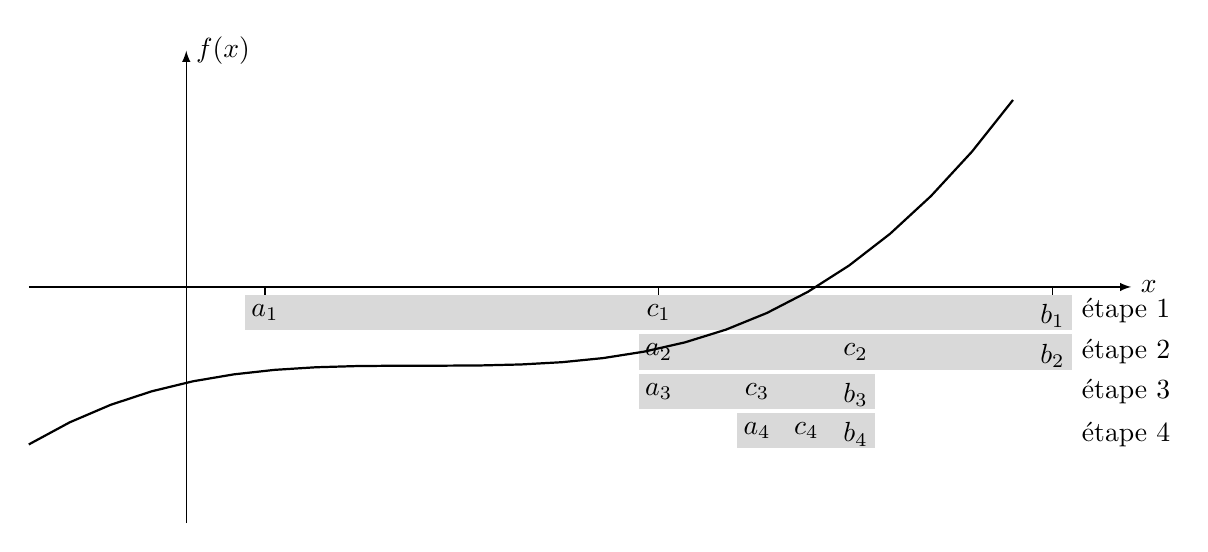
\begin{tikzpicture}
  \draw[-latex] (0,0) -- (14,0) node[right]{$x$ };
  \draw[-latex] (2,-3) -- (2,3) node[right]{$f(x)$ };
  \fill[gray!30] (2.75, -0.1) rectangle (13.25, -0.55) (13.25, -0.3) node[right, black] {étape 1};
  \fill[gray!30] (7.75, -0.6) rectangle (13.25, -1.05) (13.25, -0.825) node[right, black] {étape 2};
  \fill[gray!30] (7.75, -1.1) rectangle (10.75, -1.55) (13.25, -1.325) node[right, black] {étape 3};
  \fill[gray!30] (9, -1.6) rectangle (10.75, -2.05) (13.25, -1.875) node[right, black] {étape 4};
  \draw[thick, domain=0:12.5] plot (\x,{((\x-5)/5)^3-1}); 
  \draw (3, 0) -- ++(0, -0.1) node[below]{$a_1$};
  \draw (13, 0) -- ++(0, -0.1) node[below](b1){$b_1$};
  \draw (8, 0) -- ++(0, -0.1) node[below](c1){$c_1$};
  \draw[] (8, -0.6) node[below, ](a2){$a_2$};
  \draw[] (13, -0.6) node[below, ](b2){$b_2$};
  \draw[] (10.5, 0)  ++(0, -0.6) node[below, ](c2){$c_2$};
  \draw[] (8, -1.1) node[below, ](a3){$a_3$};
  \draw[] (10.5, -1.1) node[below, ](b3){$b_3$};
  \draw[] (9.25, 0)  ++(0, -1.1) node[below, ](c3){$c_3$};
  \draw[] (9.25, -1.6) node[below, ](a4){$a_4$};
  \draw[] (10.5, -1.6) node[below, ](b4){$b_4$};
  \draw[] (9.875, 0)  ++(0, -1.6) node[below, ](c4){$c_4$};
 
\end{tikzpicture}
\end{center}

On peut implémenter cette méthode avec la fonction python suivante :
\begin{minted}{python}
def zero_dicho(f, a, b, eps):
  while b-a > eps:    # Tant que la taille de l'intervalle est trop grande
    c = (a+b)/2       # Calcule le milieu de l'intervalle
    if f(c)*f(a)<0:   # Est-ce que la fonction change de signe sur [a,c]
      b=c             # Si oui, c devient b
    else:
      a=c             # Sinon c devient a car f change de signe sur [c,b]
  return (a+b)/2      # Renvoie le milieu de l'intervalle
\end{minted}

Le problème de la partie~\ref{sub:determiner_l_etat_final} peut alors se résoudre de la manière suivante
\begin{minted}{python}
def f(x):
    c1 = 1e-2
    V1 = 30e-3
    c2 = 1
    V2 = 20e-3
    V = V1+V2
    c0 = 1
    K = 10**12.6
    return (c0*V)**4*x/((c1*V1-x)*(c2*V2-4*x)**4)-K
print(zero_dicho(f,0, 3e-4, 1e-19)) 
\end{minted}
On trouve alors $\xi_f=\SI{2.999999999962297e-4}{\mole}$. On voit donc que l'on n'a pas commis une grosse erreur en considérant que la réaction était totale. 
\end{document} 
%%% Local Variables: 
%%% mode: latex
%%% LaTeX-command: "latex -shell-escape"
%%% End: 
